\chapter{Optimisation results}
\label{chap:optimisation-results}

Testing the impact of my optimisations presents three primary
difficulties:

\begin{enumerate}
\item The optimisation is ``incomplete'', in the sense that we likely
  fuse too aggressively (as outlined in \cref{sec:whentofuse}), and
  are too conservative about duplicating trivial computation.

\item There is not yet a way to execute \LO{} code in a performant
  manner.  The \LO{} compiler has an interpreter, but its performance
  characteristics are very different from parallel hardware -- for
  example, variable bindings carry great overhead.

  The compiler also has a code generator which generates strictly
  sequential C code.  The resulting C code uses very naïve memory
  management, however.  In particular it copies arrays very often when
  entering loops, although this might put the fusion optimisation in a
  better light, as it will reduce the sum number of loops.

\item Finally, fusion, which is our primary optimisation, does not
  really reduce the number of discrete computation steps necessary to
  execute the program.  The purpose of our fusion optimisation is to
  increase parallelism and reduce the number of discrete GPU kernels,
  which is not something that will benefit the sequential code
  generated by our code generator.
\end{enumerate}

Nevertheless, I will make an attempt at evaluating the impact of the
fusion optimisation.  This will primarily be in the form of manual
inspection of program structure befor and after optimisation, with
comments on the quality of the result.  The reader can be assured that
said inspection of thousands of lines of machine-generated code was
enormously tedious.

Six programs will be used for evaluation: three relatively simple,
artificial benchmarks, and three real-world financial programs that
have been manually translated from C++ to what we consider
``idiomatic'' \LO{}\footnote{Or at least as much as it makes sense to
  talk about an ``idiomatic'' style for a language whose users are its
  designers.}.  I present runtimes for these programs in
\cref{sec:runtime-results}.

The artificial benchmarks are the following:

\begin{description}
% data/benchmarks/BlackScholes.l0
\item[P0] Black-Scholes\cite{black1973pricing} pricing computation.

% data/tests/MatMultFun.l0
\item[P1] Matrix multiplication written in a functional style (i.e, no
  use of \texttt{loop} and \texttt{let-with}).

% data/benchmarks/BabyBear.l0
\item[P2] BabyBear - a tiny ursine.
\end{description}

And the real world benchmarks:

\begin{description}
% data/benchmarks/CalibLexiFi.l0
\item[R0] Parameter calibration program.

% data/benchmarks/PricingLexiFi.l0
\item[R1] Pricing program.

% data/benchmarks/HiperfitEgCos.l0
\item[R2] Some C++ mess we got from Nordea.
\end{description}

\begin{figure}
\begin{tabular}{p{1.6cm}|p{1.6cm}|p{1.6cm}|p{1.6cm}|p{1.6cm}|p{1.6cm}}
\multicolumn{2}{c}{\textbf{P0}} & \multicolumn{2}{c}{\textbf{P1}} & \multicolumn{2}{c}{\textbf{P2}} \\
\hline
Before & After & Before & After & Before & After \\
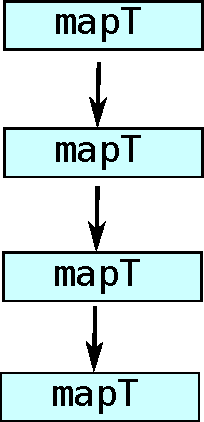
\includegraphics[width=1.6cm]{img/BlackScholes-unfused.pdf} &
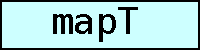
\includegraphics[width=1.6cm]{img/BlackScholes-fused.pdf} &
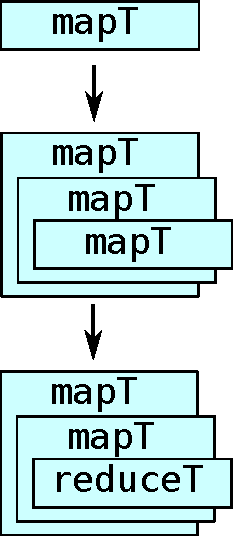
\includegraphics[width=1.6cm]{img/MatMultFun-unfused.pdf} &
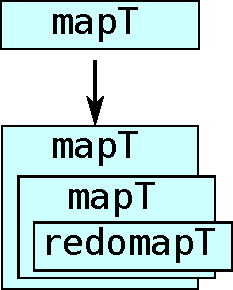
\includegraphics[width=1.6cm]{img/MatMultFun-fused.pdf} &
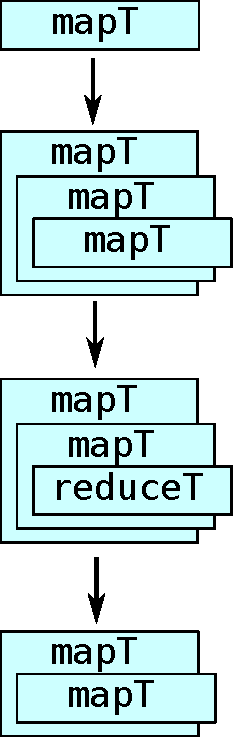
\includegraphics[width=1.6cm]{img/BabyBear-unfused.pdf} &
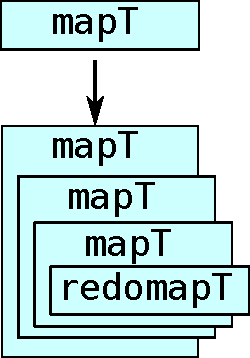
\includegraphics[width=1.6cm]{img/BabyBear-fused.pdf}
\end{tabular}
\caption{Artificial benchmark dataflows, before and after optimisation}
\label{fig:artificial-dataflows}
\end{figure}

\begin{figure}
\begin{center}
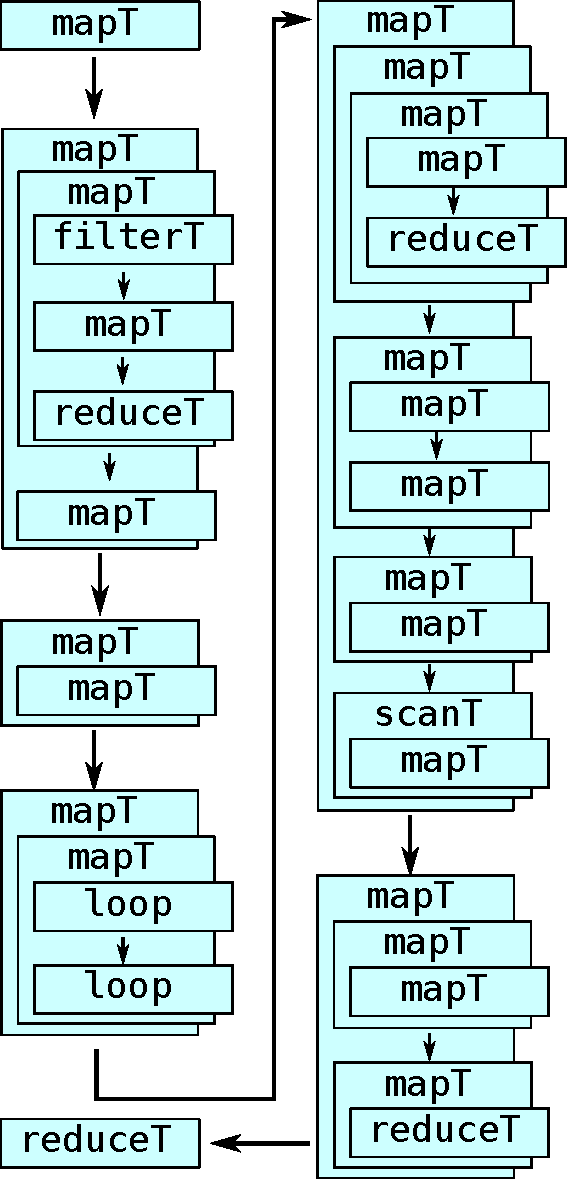
\includegraphics[width=3.2cm]{img/PricingLexiFi-unfused.pdf}
\hspace{1cm}
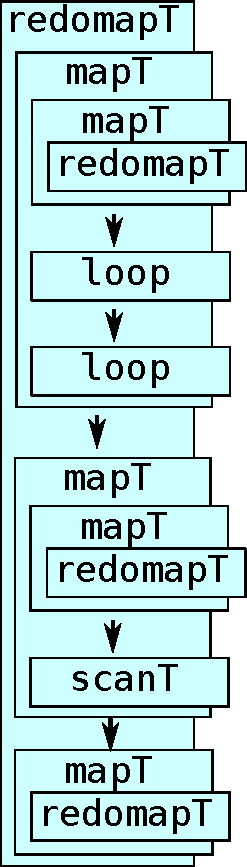
\includegraphics[width=1.6cm]{img/PricingLexiFi-fused.pdf}
\end{center}
\caption{R1 benchmark dataflow, before and after optimisation}
\label{fig:r1-dataflow}
\end{figure}

\begin{figure}
\begin{center}
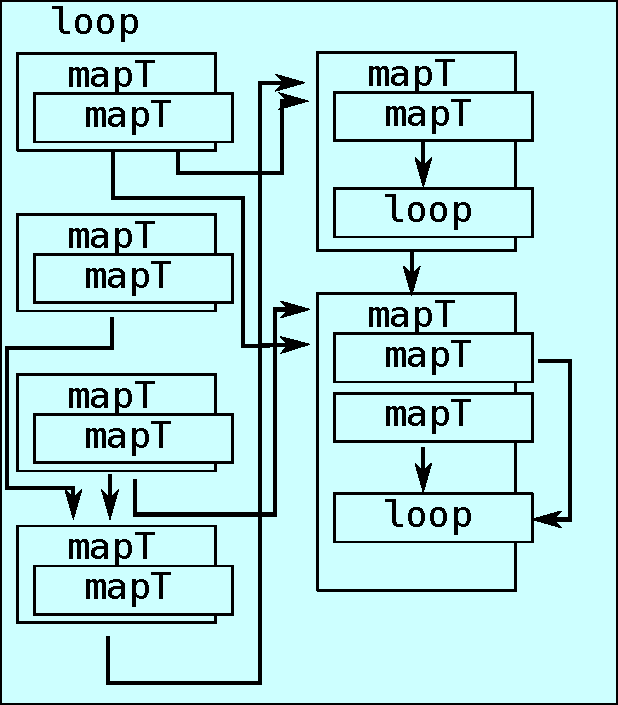
\includegraphics[width=3.2cm]{img/HiperfitEgCos-unfused.pdf}
\hspace{1cm}
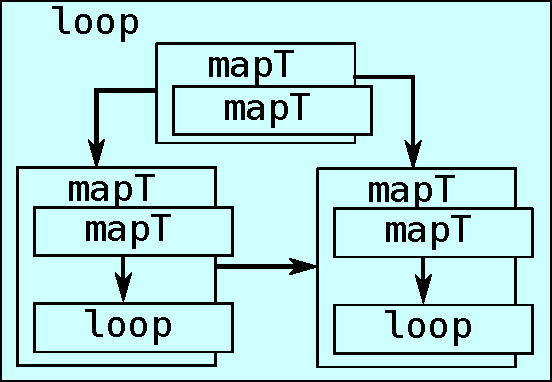
\includegraphics[width=3.2cm]{img/HiperfitEgCos-fused.pdf}
\end{center}
\caption{R2 benchmark dataflow, before and after optimisation}
\label{fig:r2-dataflow}
\end{figure}

\begin{figure}
\begin{center}
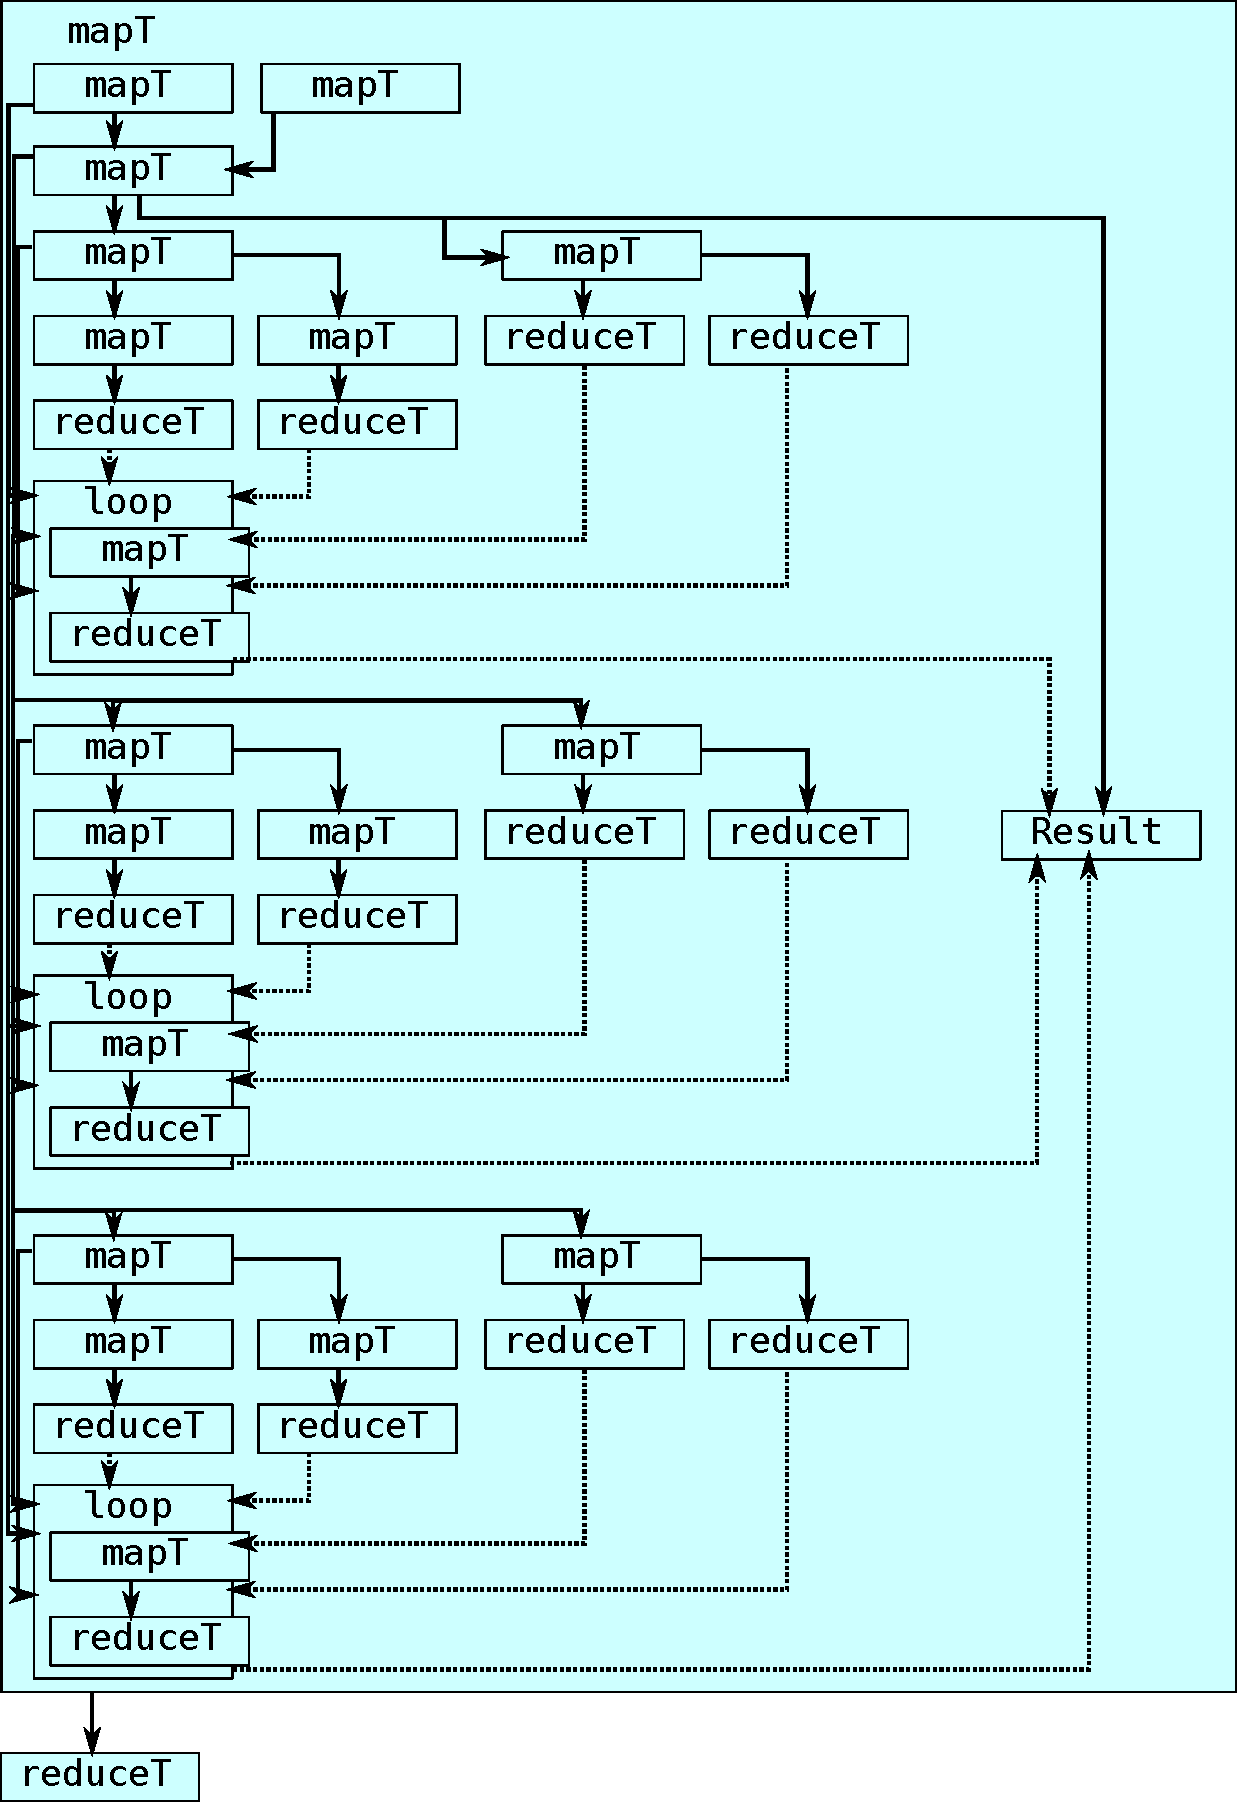
\includegraphics[width=9.6cm]{img/CalibLexiFi-unfused.pdf}
\end{center}
\caption{R0 benchmark dataflow, before optimisation}
\label{fig:r2-dataflow-unfused}
\end{figure}

\begin{figure}
\begin{center}
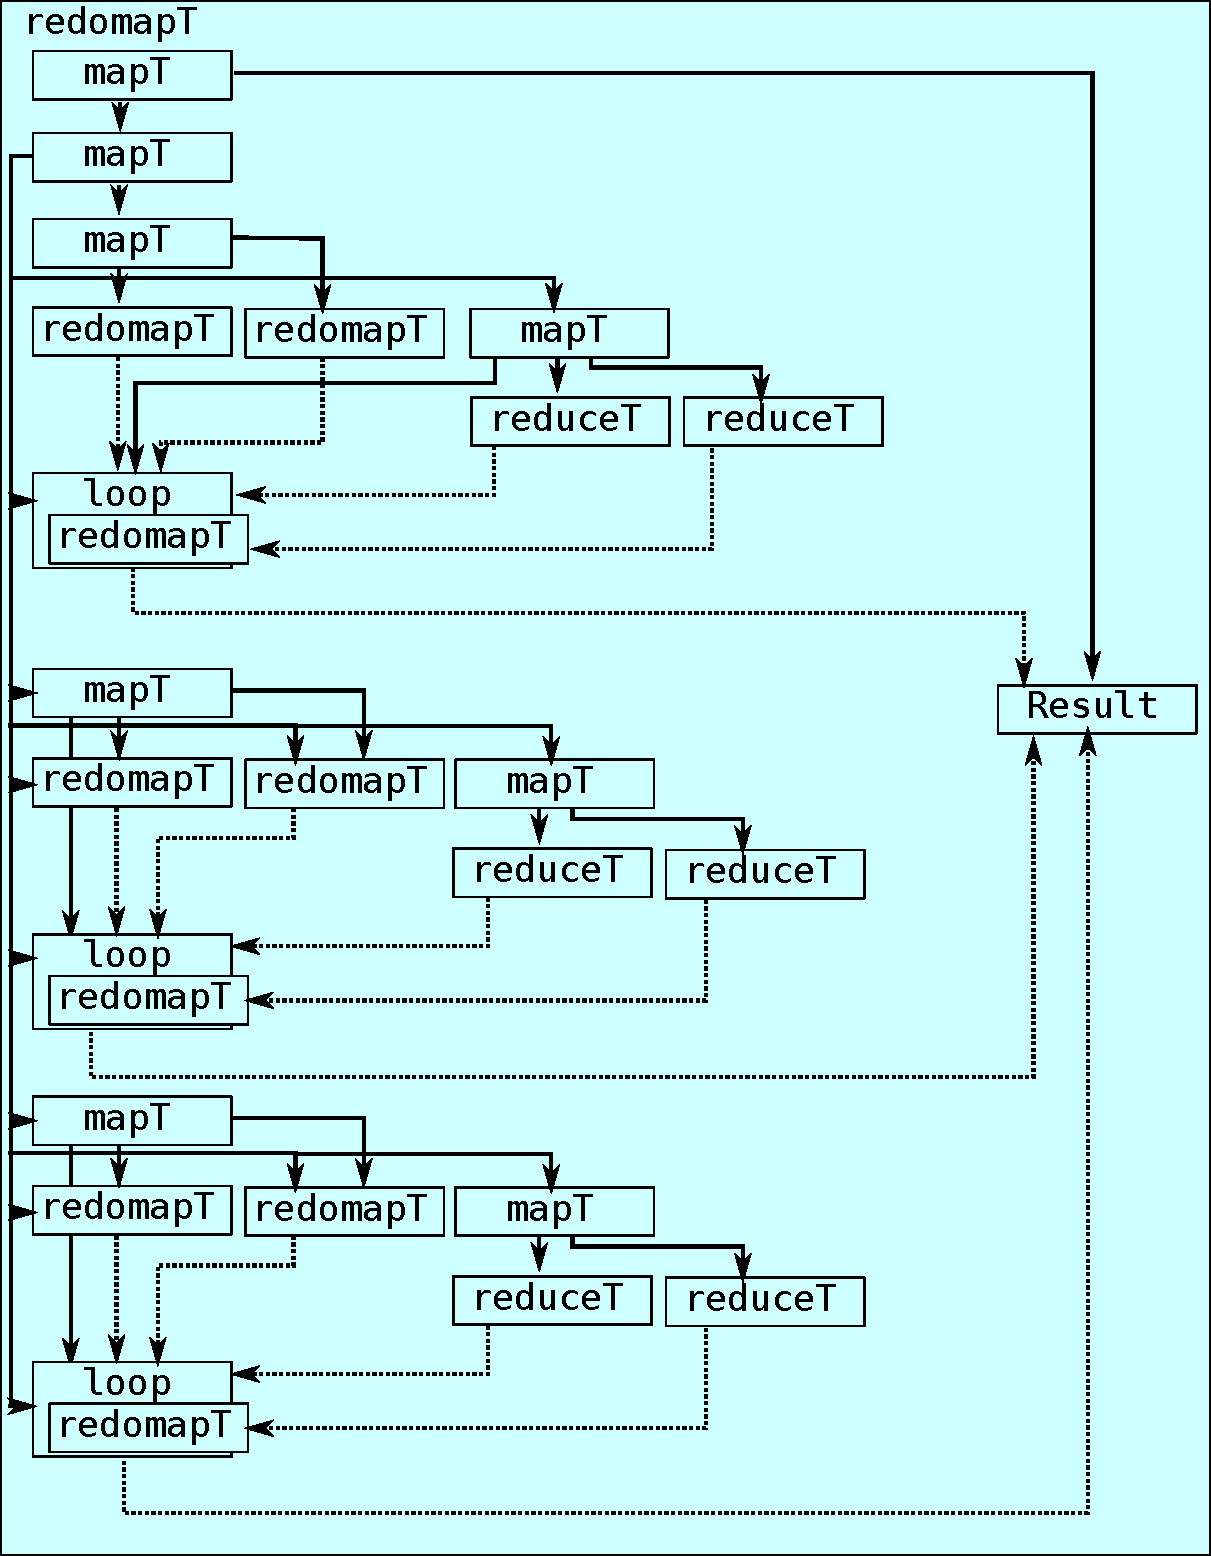
\includegraphics[width=9.6cm]{img/CalibLexiFi-fused.pdf}
\end{center}
\caption{R0 benchmark dataflow, after optimisation}
\label{fig:r2-dataflow-fused}
\end{figure}

\section{Runtime results}
\label{sec:runtime-results}

%%% Local Variables: 
%%% mode: latex
%%% TeX-master: "thesis.tex"
%%% End: 
